% Created 2021-12-08 Wed 18:34
% Intended LaTeX compiler: pdflatex
\documentclass[11pt]{article}
\usepackage[utf8]{inputenc}
\usepackage[T1]{fontenc}
\usepackage{graphicx}
\usepackage{grffile}
\usepackage{longtable}
\usepackage{wrapfig}
\usepackage{rotating}
\usepackage[normalem]{ulem}
\usepackage{amsmath}
\usepackage{textcomp}
\usepackage{amssymb}
\usepackage{capt-of}
\usepackage{hyperref}
\usepackage{amsfonts} \usepackage{amssymb} \usepackage{mathtools} \usepackage{ upgreek }
\author{Logan Hunt}
\date{\today}
\title{Final Project: Game of Life}
\hypersetup{
 pdfauthor={Logan Hunt},
 pdftitle={Final Project: Game of Life},
 pdfkeywords={},
 pdfsubject={},
 pdfcreator={Emacs 27.2 (Org mode 9.4.4)}, 
 pdflang={English}}
\begin{document}

\maketitle

\section{Description}
\label{sec:orgee5348a}
From \href{https://mathworld.wolfram.com/CellularAutomaton.html}{Wolfram MathWorld}:

\begin{quote}
A cellular automaton is a collection of "colored" cells on a grid of specified shape that evolves through a number of discrete time steps according to a set of rules based on the states of neighboring cells. The rules are then applied iteratively for as many time steps as desired. 
\end{quote}

Conway's Game of Life is one such automaton. In the Game of Life, the rules for each cell are as follows (from \href{https://en.wikipedia.org/wiki/Conway\%27s\_Game\_of\_Life}{Wikipedia}):

\begin{quote}
\begin{enumerate}
\item Any live cell with fewer than two live neighbours dies, as if by underpopulation.
\item Any live cell with two or three live neighbours lives on to the next generation.
\item Any live cell with more than three live neighbours dies, as if by overpopulation.
\item Any dead cell with exactly three live neighbours becomes a live cell, as if by reproduction.
\end{enumerate}
\end{quote}

To help visualize this automaton I created a script to go through the output of my Game of Life simulation and compile a video with ffmpeg. As an example, I've uploaded the output of a simulation with a 1920x1080 grid of cells with 1000 iterations \href{https://www.youtube.com/watch?v=N\_aUWYNqpeY}{to YouTube}. Each cell that is white is alive and each black cell is dead.

There are four implementations of Conway's Game of Life in this project; a serial implementation, a distributed memory implementation (in OpenMPI), a shared memory implementation (in OpenMP), and a GPU implementation (in Cuda). 

A timing study is performed on each implementation by calculating the elapsed time of the program given varying sizes of initial grids and, in the shared and distributed memory versions, a different number of cores. In each, both the time it takes to compute the next iteration and the total wall clock time are measured.

\section{Performance analysis (of Game of Life iteration time)}
\label{sec:org1f7f2b6}
Results can be found on a \href{https://docs.google.com/spreadsheets/d/1QxCsyMFzk67Qpuv-xZ-tRny4jHMebXTrdq5ncc7C4Tw/edit?usp=sharing}{Google Sheet}
\subsection{Shared memory vs distributed memory}
\label{sec:org9f5d8c9}
\subsubsection{Runtime}
\label{sec:org9209384}
In runtime, both implementations have the same property of decreasing over an increasing number of cores in all problem sizes (as one would certainly hope). As the problem size increases, the overall differences in the runtimes of each implementation also decreases; meaning they follow the same trends. This can be shown in the runtimes for both implmentations running on a small grid and a large grid:

\begin{center}
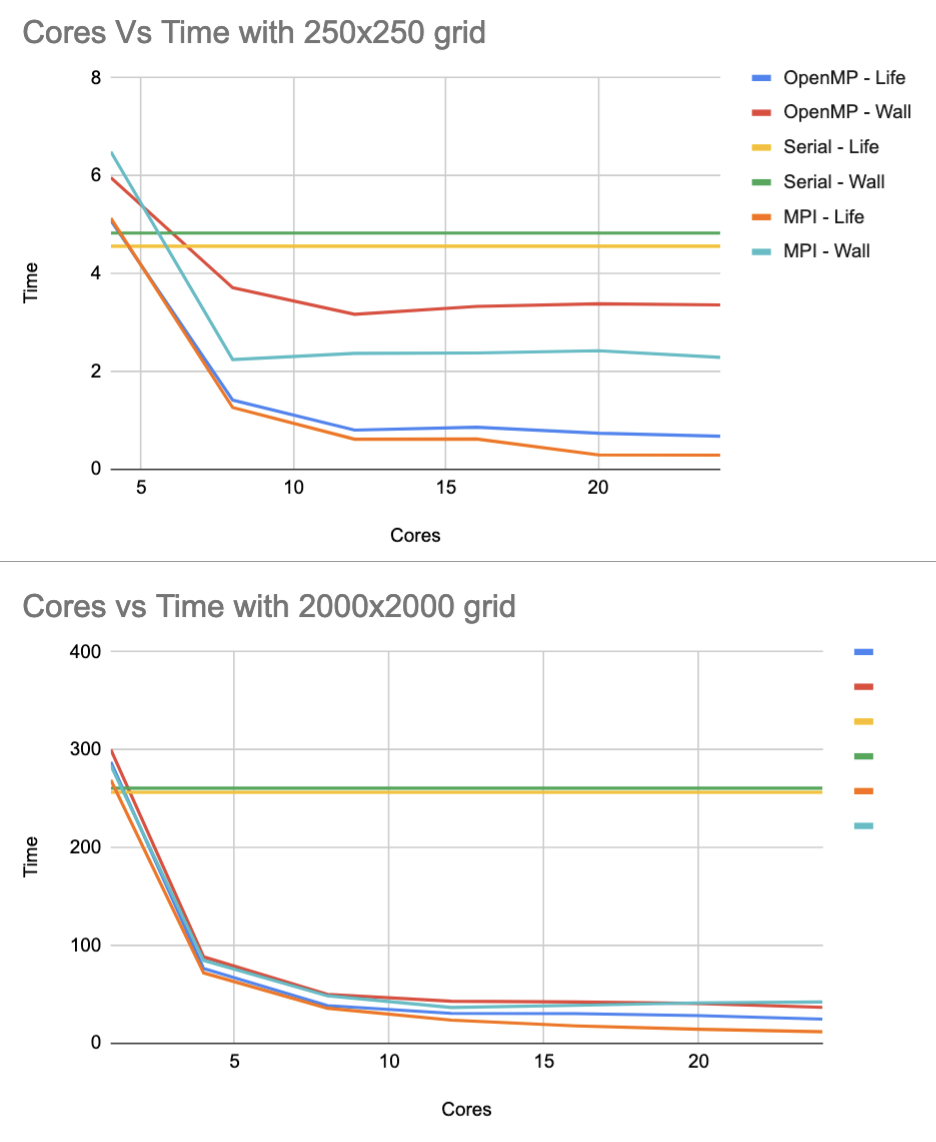
\includegraphics[width=8cm]{./cores-vs-runtimes.png}
\end{center}

Both seem to converge to some rational function. Using an online regression calculator it was found that the MPI Life Computation (iteration computation time only) runtime follows the function \(t(p)=\frac{274.449}{p^{0.985}}\) with a correlation coefficient of \(r=-0.999892441\). Since \(t\) is very close to being a rational function of \(p\), we know that the runtime fits to what could be expected: \(T_{\text{parallel}} = \frac{T_{\text{serial}}}{p}\).

\subsubsection{Speedup}
\label{sec:org3812f4f}
In speedup, both implementations tend to increase over an increasing number of cores in all problem sizes. However, it doesn't strictly increase. With some numbers of cores in the shared memory implementation, the speedup actually decreases from its predecessor. 

\begin{center}
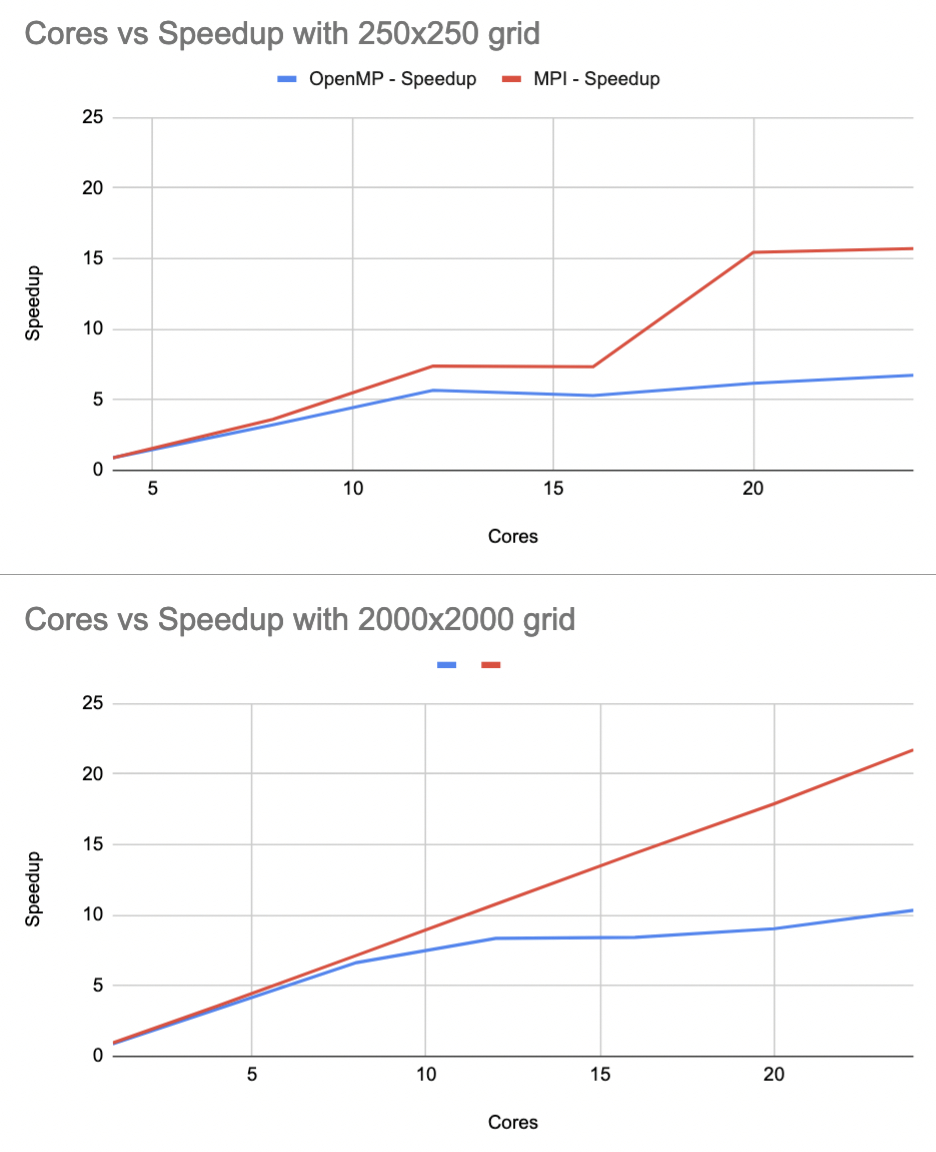
\includegraphics[width=10cm]{./speedups-vs-cores.png}
\end{center}


\subsubsection{Efficiency}
\label{sec:org477fbb5}
Efficiency is the ratio of speedup to \(p\) processors (\(E = \frac{S}{p}\)), so it can be thought of as the derivative of the speedup. Thus efficiency can be measured without plotting it explicitly.

By definition, a program is "strongly scalable" if it can keep its efficiency constant over a varying input size. In the results, it can be seen that the slope of the Distributed Memory Life Computation Time line tends to be constant, meaning that the efficiency is also constant. Thus, the MPI version is strongly scalable.

However, the shared memory (OpenMP) implementation does not seem to be perfectly strongly scalable. As the problem size varies, the speedup does not follow a constant slope. Instead, it tends to match the efficiency of the MPI implemenation until some point where the slope drops off. 

Theoretically, the OpenMP implementation should be just as strongly scalable as the MPI implementation. One reason overhead could be present is in thread scheduling. 

\subsection{CUDA Implementation}
\label{sec:org31daf97}
\subsubsection{Runtime}
\label{sec:orgb6b22ab}
For the CUDA implementation, different grid sizes are used to measure the iteration time as well as the wall time. Again, 1000 iterations are used for the timing study.

\begin{center}
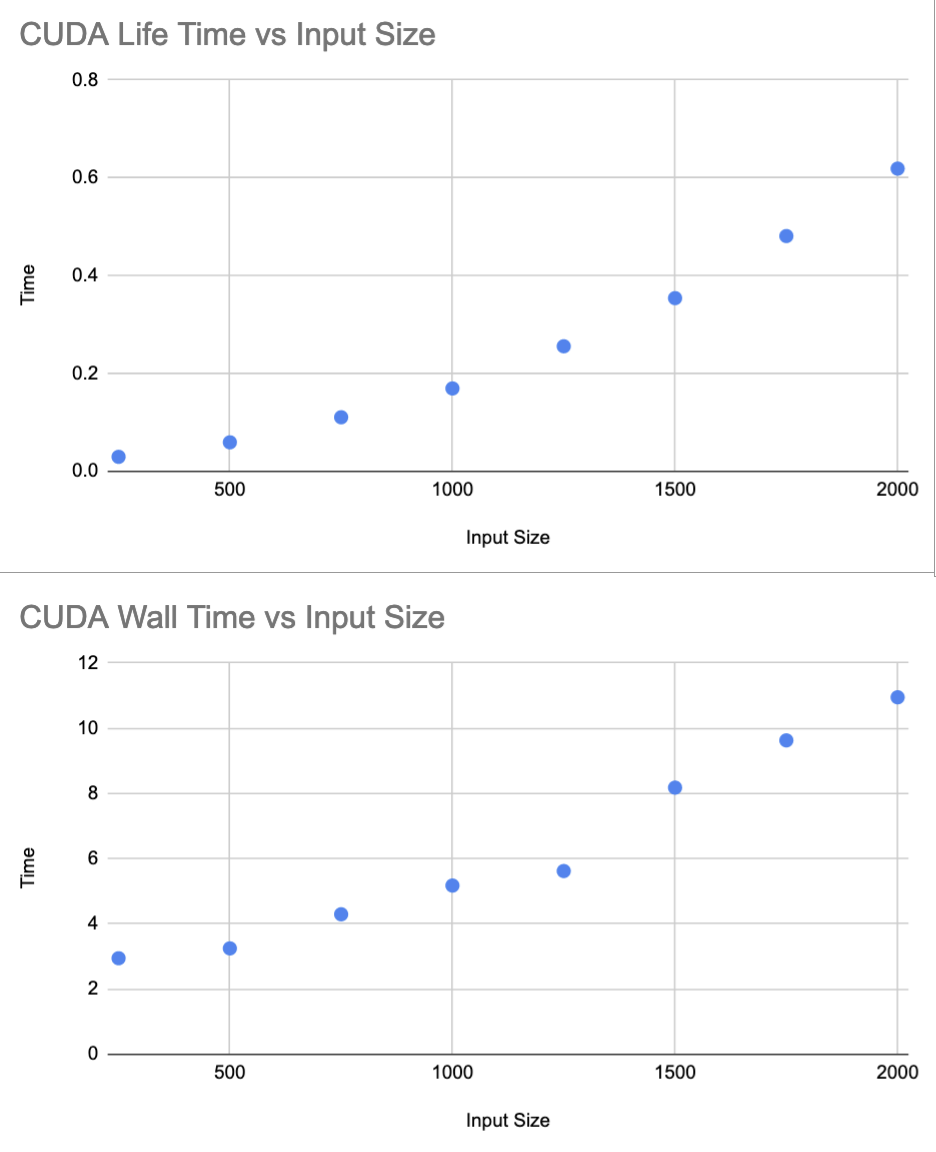
\includegraphics[width=8cm]{./cuda-times.png}
\end{center}

Using an online regression calculator again, it was found that the runtime as a function of input size can be expressed with by \(t(n) = (1.486)(10^{-7})n^2 + (1.328)(10^{-6})n + 0.02151\) with a correlation coefficient \(r = 0.9999278678\).

Since the number of cores is constant, we would hope to see a quadratic increase in the runtime as the input size grows. This is because the number of cells increases with \((\text{input size})^2\).

Indeed, this is what we see.

\subsubsection{Speedup}
\label{sec:org888d520}
The speedup of the cuda implementation as input size increases tends to follow a logarithmic curve, plateuing after around \(n=1000\). While I am not entirely sure why it follows this trend, I guess it might have to do with the warp scheduling.

\begin{center}
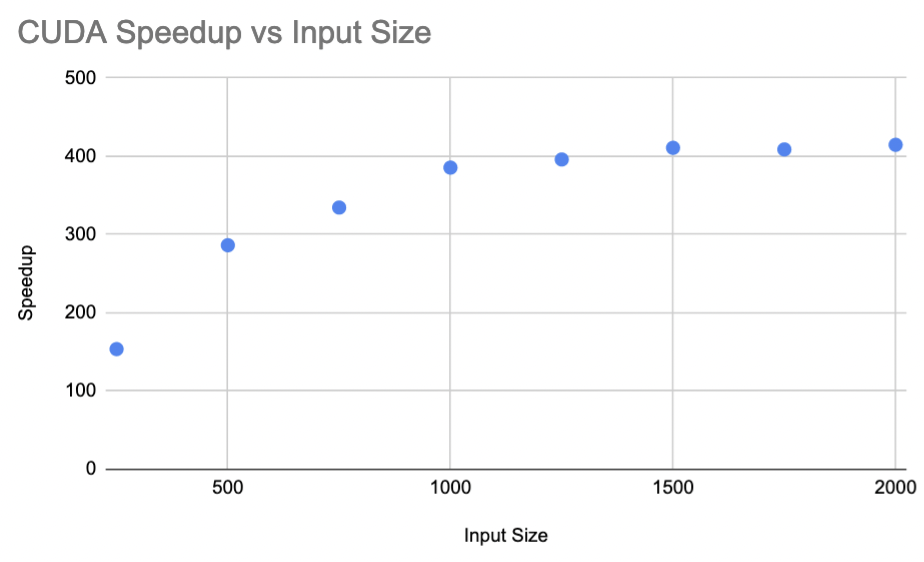
\includegraphics[width=8cm]{./cuda-speedup.png}
\end{center}

\subsubsection{Efficiency}
\label{sec:org530b4aa}
Since the core count on the K80 is constant (4992 CUDA cores), the efficiency can be calculated by \(E = \frac{S}{4992}\). As the efficiency is just a constant multiplied by the speedup, the efficiency graph will just be a scaled version of the speedup graph. As such the efficiency will not be constant over different input sizes since the speedup isn't, and thus the CUDA implementation is not strongly scalable.
\end{document}
